\chapter{SQL DCL}\label{cha:dcl}

\section{Was ist DCL?}
Die \emph{Data Control Language} (DCL), auch Datenüberwachungssprache genannt, ist eine Teilmenge der Structured Query Language (SQL) und ermöglicht es Datenbankadministratoren, den Sicherheitszugriff auf relationale Datenbanken zu konfigurieren. Eine „vollwertige“ SQL-Datenbank enthält umfassende Regelungen über die Vergabe von Rechten für den Zugriff auf Objekte (Tabellen, einzelne Felder, interne Funktionen usw.).

DCL ist die einfachste der SQL-Teilmengen, da sie nur aus drei Befehlen besteht: GRANT, REVOKE und DENY. Zusammen bieten diese drei Befehle Administratoren die Flexibilität, Datenbankberechtigungen äußerst detailliert festzulegen und zu entfernen. Es gibt auch einige Software-Hersteller die den Begriff DCL nicht verwenden, stattdessen werden da die Berechtigungsbefehle zur DDL gezählt. 

\section{Wer kann den Benutzern diese Rechte gewähren oder von ihnen entfernen?}
Nur Datenbankadministratoren (DBAs) oder Datenbankeigentümer sind berechtigt, den Benutzern Berechtigungen zu erteilen oder diese zu entfernen. Andere Benutzer müssen ausdrücklich zu einzelnen Handlungen ermächtigt werden. 

\section{Privilegien}
Wenn mehrere Benutzer auf Datenbankobjekte zugreifen können, kann die Berechtigung für diese Objekte mit Berechtigungen gesteuert werden. Jedes Objekt hat einen Besitzer. Berechtigungen steuern, ob ein Benutzer ein Objekt ändern kann, dessen Eigentümer ein anderer Benutzer ist. Berechtigungen werden entweder vom Instanz Administrator, einem Benutzer mit der Berechtigung ADMIN oder für Berechtigungen für ein bestimmtes Objekt vom Eigentümer des Objekts erteilt oder entzogen.

\subsection{System Privilegien}
Systemberechtigungen sind Berechtigungen, mit denen Benutzer bestimmte Funktionen ausführen können, die sich mit der Verwaltung der Datenbank und des Servers befassen. Die meisten verschiedenen Arten von Berechtigungen, die von den Datenbankanbietern unterstützt werden, fallen unter die Kategorie der Systemberechtigungen. Nur der Instanz Administrator oder ein Benutzer mit ADMIN - Berechtigungen kann Systemberechtigungen erteilen oder entziehen. 

Beispiele für System Privilegien:

\begin{itemize}
    \item \emph{CREATE USER} - Wenn die CREATE USER-Berechtigung einem Datenbankbenutzer erteilt wird, kann dieser Datenbankbenutzer neue Benutzer in der Datenbank erstellen. 
    \item \emph{CREATE TABLE} - Mit der CREATE TABLE-Berechtigung, die einem Datenbankbenutzer erteilt wird, kann dieser Datenbankbenutzer Tabellen in seinem eigenen Schema erstellen. Diese Art von Berechtigungen steht auch für andere Objekttypen zur Verfügung, z. B. gespeicherte Prozeduren und Indizes.
    \item \emph{CREATE SESSION} - Wenn die CREATE SESSION-Berechtigung einem Datenbankbenutzer erteilt wird, kann dieser Datenbankbenutzer eine Verbindung zur Datenbank herstellen. 
\end{itemize}

\subsection{Objekt Privilegien}
Ein Objektprivileg ist das Recht, eine bestimmte Aktion an einem Datenbankobjekt auszuführen oder auf das Datenbankobjekt eines anderen Benutzers zuzugreifen - wobei es sich bei Datenbankobjekten um Tabellen, gespeicherte Prozeduren, Indizes usw. handelt. Der Eigentümer eines Objekts verfügt über alle Objektberechtigungen für dieses Objekt, und diese Berechtigungen können nicht widerrufen werden. Der Eigentümer des Objekts kann anderen Datenbankbenutzern Objektberechtigungen für dieses Objekt erteilen. Ein Benutzer mit ADMIN - Berechtigungen kann Objektberechtigungen von Benutzern erteilen und entziehen, die nicht Eigentümer der Objekte sind, für die die Berechtigungen erteilt wurden. 

Beispiele für Objekt Privilegien:

\begin{itemize}
    \item \emph{SELECT} - Ermöglicht einem Benutzer die Auswahl aus einer Tabelle, einer Sequenz, einer Ansicht usw. 
    \item \emph{UPDATE} - Ermöglicht einem Benutzer das Aktualisieren einer Tabelle. 
    \item \emph{DELETE} - Ermöglicht einem Benutzer das Löschen aus einer Tabelle. 
\end{itemize}

\begin{figure}[h]
    \centering
    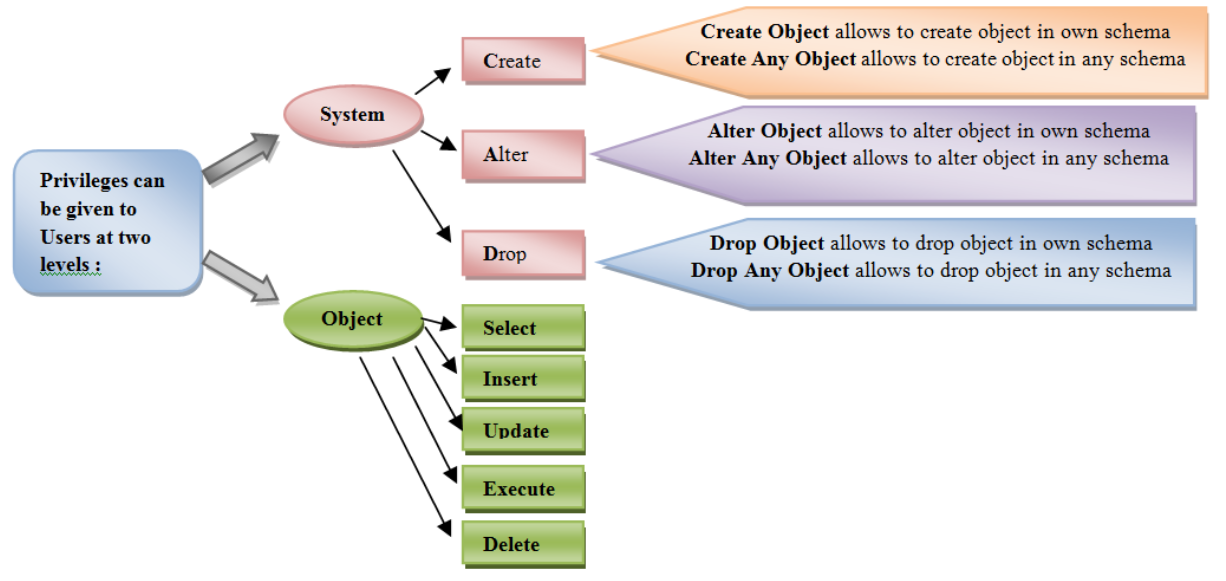
\includegraphics[width=.95\textwidth]{Content/images/dcl/privileges.png}
    \caption{Privilegien}
    \label{fig:privilegien}
 \end{figure}

\section{Hinzufügen von Berechtigungen mit GRANT}
Der Befehl GRANT wird von Administratoren verwendet, um einem Datenbankbenutzer neue Berechtigungen hinzuzufügen. Es hat eine sehr einfache Syntax, die wie folgt definiert ist:

\subsection{Syntax}
\begin{figure}[h]
    \centering
    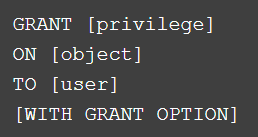
\includegraphics[width=.30\textwidth]{Content/images/dcl/syntax_grant.png}
    \caption{GRANT Syntax}
    \label{fig:syntax-grant}
 \end{figure}

Hier ist der Überblick über die einzelnen Parameter, die Sie mit diesem Befehl bereitstellen können:

\begin{itemize}
    \item \emph{Privilege}: Dies kann entweder das Schlüsselwort ALL (um eine Vielzahl von Berechtigungen zu erteilen) oder eine bestimmte Datenbankberechtigung oder eine Reihe von Berechtigungen sein. Beispiele sind CREATE DATABASE, SELECT, INSERT, UPDATE, DELETE, EXECUTE, CREATE VIEW usw.
    \item \emph{Object}: Kann ein beliebiges Datenbankobjekt sein. Die gültigen Berechtigungsoptionen hängen vom Typ des Datenbankobjekts ab, das Sie in diese Klausel aufnehmen. In der Regel handelt es sich bei dem Objekt entweder um eine Datenbank, eine Funktion, eine gespeicherte Prozedur, eine Tabelle oder eine Ansicht.
    \item \emph{User}: Kann ein beliebiger Datenbankbenutzer sein. Sie können in dieser Klausel auch eine Rolle für den Benutzer ersetzen, wenn Sie die rollen basierte Datenbanksicherheit nutzen möchten.Verwenden Sie das Schlüsselwort PUBLIC, um alle Benutzer anzugeben.
\end{itemize}

\subsection{With grant option and With admin option}
Es gibt einen sehr deutlichen Unterschied, und es ist wichtig, die Auswirkungen der Verwendung von entweder "with grant option" oder "with admin option" sorgfältig zu prüfen. Diese Option gibt die Kontrolle über die Datenbankberechtigungen von einem einzelnen Datenbankbesitzer an mehrere Benutzer weiter. Dies muss sorgfältig kontrolliert werden, um die richtige Sicherheit zu gewährleisten.

Die Verwendung der Optionen "with admin" und "with grant" wird als Oracle-gefährlich eingestuft, da es bei unsachgemäßer Verwaltung zu unbeabsichtigten Nebenwirkungen kommen kann, die zu einer Sicherheitslücke führen. Sowohl die Optionen 'with grant' als auch 'with admin' dienen dazu, die zentrale Sicherheitskontrolle aufzugeben, gelten jedoch für verschiedene Arten von Berechtigungen.

\subsubsection{With Grant Option}
\begin{itemize}
    \item Nur für Objektprivilegien, keine Systemprivilegien.
    \item Nur die Person, die das Privileg erteilt hat, kann das Privileg widerrufen.
    \item Aufgehobene Berechtigungen können "kaskadieren", sodass der erste Berechtigte viele nachfolgende Berechtigungen widerrufen kann.
\end{itemize}

\subsubsection{With admin option}
\begin{itemize}
    \item Nur für Systemprivilegien, keine Objektprivilegien.
\end{itemize}

\section{Datenbankzugriff widerrufen mit REVOKE}
Der Befehl REVOKE wird verwendet, um den Datenbankzugriff von einem Benutzer zu entfernen, dem zuvor ein solcher Zugriff gewährt wurde. Die Syntax für diesen Befehl ist wie folgt definiert:

\subsection{Syntax}
\begin{figure}[h]
    \centering
    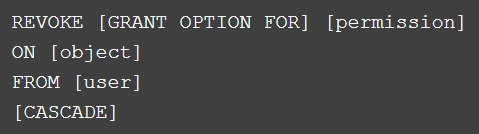
\includegraphics[width=.30\textwidth]{Content/images/dcl/syntax_revoke.png}
    \caption{REVOKE Syntax}
    \label{fig:syntax-revoke}
 \end{figure}

\begin{itemize}
    \item \emph{Permission}: Gibt die Datenbankberechtigungen an, die vom identifizierten Benutzer entfernt werden sollen. Der Befehl widerruft sowohl GRANT- als auch DENY - Zusicherungen, die zuvor für die identifizierte Berechtigung gemacht wurden.
    \item \emph{Object, User}: Das gleiche wie beim GRANT Kommando.
    \item \emph{Grant option for}: Die Klausel entfernt die Fähigkeit des angegebenen Benutzers, anderen Benutzern die angegebene Berechtigung zu erteilen. Anmerkung: Wenn Sie die Klausel GRANT OPTION FOR in eine REVOKE - Anweisung aufnehmen, wird die primäre Berechtigung nicht widerrufen. Diese Klausel widerruft nur die GRANT Fähigkeit.
    \item \emph{Cascade}: Entzieht allen Benutzern, denen der angegebene Benutzer die Berechtigung erteilt hat, die angegebene Berechtigung.
\end{itemize}

\section{Verweigerung des Datenbankzugriffs mit DENY}
Mit dem Befehl DENY wird explizit verhindert, dass ein Benutzer eine bestimmte Berechtigung erhält. Dies ist hilfreich, wenn ein Benutzer Mitglied einer Rolle oder Gruppe ist, der eine Berechtigung erteilt wurde, und Sie möchten verhindern, dass dieser einzelne Benutzer die Berechtigung erbt, indem Sie eine Ausnahme erstellen. Die Syntax für diesen Befehl lautet wie folgt:

\begin{figure}[h]
    \centering
    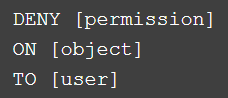
\includegraphics[width=.30\textwidth]{Content/images/dcl/syntax_deny.png}
    \caption{DENY Syntax}
    \label{fig:syntax-deny}
 \end{figure}

Die Parameter für den Befehl DENY sind identisch mit denen für den Befehl GRANT.

\section{Rollen}
Rollen können als Bündel oder Paket von Berechtigungen definiert werden. Wenn dem Benutzer automatisch eine Rolle zugewiesen wird, werden alle untergeordneten Berechtigungen auch dem Benutzer zugewiesen. Ähnliches gilt für den Widerruf. Der Hauptvorteil des Erstellens von Rollen besteht darin, dass in einer Mehrbenutzerumgebung, in der mehrere Berechtigungen auf einmal erteilt oder widerrufen werden können, das Erteilen und Widerrufen von Rollen vereinfacht wird. Andernfalls würde dies viel Zeit in Anspruch nehmen, wenn dies separat erfolgt. Es ist auch möglich, einer Rolle eine weitere Rolle hinzuzufügen.

\subsection{Systemrollen}
\begin{itemize}
    \item \emph{Connect}: Create table, Create view, Create synonym, Create sequence, Create session etc.
    \item \emph{Resource}: Create Procedure, Create Sequence, Create Table, Create Trigger etc. Die Hauptverwendung der Rolle "Ressource" besteht darin, den Zugriff auf Datenbankobjekte zu beschränken
    \item \emph{DBA}: Alle System Berechtigungen.
\end{itemize}

\begin{figure}[h]
    \centering
    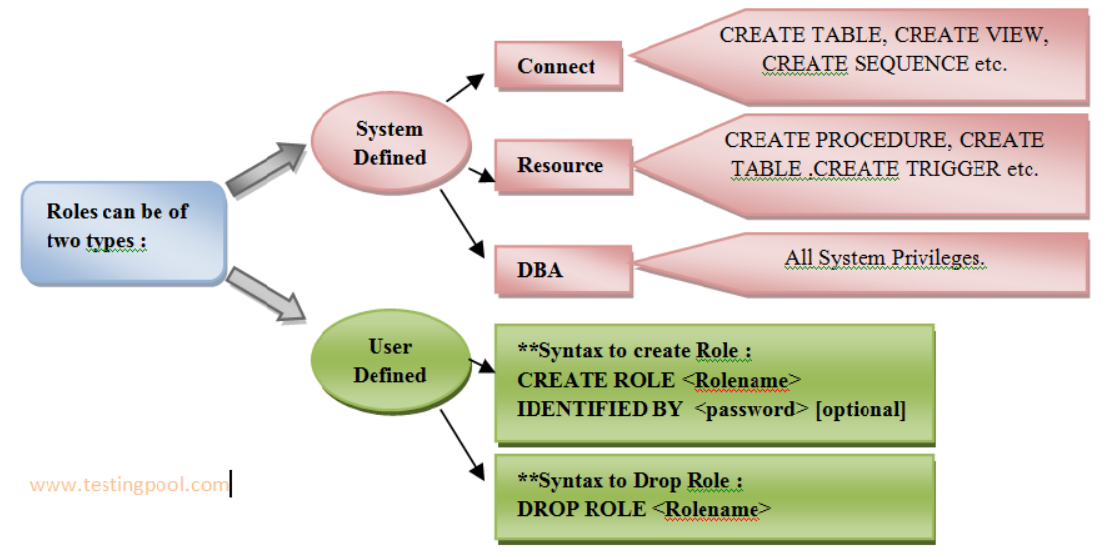
\includegraphics[width=.95\textwidth]{Content/images/dcl/rollen.png}
    \caption{Rollen}
    \label{fig:rollen}
 \end{figure}

\subsection{Rolle anlegen und zuordnen}
Zunächst muss der (Datenbankadministrator) DBA die Rolle erstellen. Dann kann der DBA der Rolle Berechtigungen und der Rolle Benutzer zuweisen.

\subsubsection{Syntax}
\begin{lstlisting}
    CREATE ROLE manager;
\end{lstlisting}

\begin{itemize}
    \item Nachdem die Rolle erstellt wurde, kann der DBA die GRANT - Anweisung verwenden, um der Rolle Berechtigungen zuzuweisen und der Rolle danach Benutzer zuzuweisen.
    \item Es ist einfacher, Berechtigungen für die Benutzer über eine Rolle zu erteilen oder zu widerrufen, als jedem Benutzer direkt eine Berechtigung zuzuweisen.
\end{itemize}

\subsubsection{Gewähren Sie einer Rolle Berechtigungen}
\begin{lstlisting}
    GRANT create table, create view
    TO manager;
\end{lstlisting}

\subsubsection{Gewähren Sie Benutzern eine Rolle}
\begin{lstlisting}
    GRANT manager to SAM, STARK;
\end{lstlisting}

\subsubsection{Berechtigung von Rolle entziehen}
\begin{lstlisting}
    REVOKE create table from manager;
\end{lstlisting}

\subsubsection{Rolle löschen}
\begin{lstlisting}
    DROP ROLE manager;
\end{lstlisting}

Zunächst wird eine Manager-Rolle erstellt, und anschließend können Manager Tabellen und Ansichten erstellen. Es gewährt dann Sam und Stark die Rolle von Managern. Jetzt können Sam und Stark Tabellen und Ansichten erstellen. Wenn Benutzern mehrere Rollen zugewiesen wurden, erhalten sie alle Berechtigungen, die mit allen Rollen verknüpft sind. Anschließend wird die Berechtigung zum Erstellen einer Tabelle mit Revoke aus der Rolle "Manager" entfernt. Die Rolle wird mit drop aus der Datenbank entfernt.

\section{User erstellen in Oracle}
Um einen User zu erstellen muss mindestens folgendes Statement ausgeführt werden.

\subsection{Syntax}
\begin{lstlisting}
    CREATE USER max_mustermann
    IDENTIFIED BY 'passme';
\end{lstlisting}

Sie müssen über das Systemprivileg CREATE USER verfügen. Wenn Sie einen Benutzer mit der Anweisung CREATE USER erstellen, ist die Berechtigungsdomäne des Benutzers leer.

\subsection{Optionale Parameter}

\subsubsection{Default Tablespace clause}
Geben Sie den default Tablespace für Objekte , die der Benutzer erstellt, immer an, wenn es möglich ist. Wenn Sie diese Klausel weglassen, werden die Objekte des Benutzers im default Tablespace der Datenbank gespeichert. Wenn für die Datenbank kein default Tablespace angegeben wurde, werden die Objekte des Benutzers im SYSTEM-Tabellenbereich gespeichert, was nicht gut ist.

\subsubsection{Temporary Tablespace clause}
Geben Sie den Tablespace oder die Tablespace - Gruppe für die temporären Segmente des Benutzers an. Wenn Sie diese Klausel weglassen, werden die temporären Segmente des Benutzers im temporären Standardtabellenbereich der Datenbank oder, falls keiner angegeben wurde, im SYSTEM-Tabellenbereich gespeichert.

Temporäre Tablespaces werden für spezielle Vorgänge verwendet, insbesondere zum Sortieren von Datenergebnissen auf der Festplatte und für Hash-Joins in SQL. Bei SQL mit Millionen von zurückgegebenen Zeilen ist der Sortiervorgang für den RAM-Bereich zu groß und muss auf der Festplatte erfolgen. In dem temporären Tablespace findet dies statt.


\subsubsection{Quota clause}
Verwenden Sie die QUOTA-Klausel, um den maximalen Speicherplatz anzugeben, den der Benutzer im Tablespace bzw. default Tablespace zuweisen kann. Mit UNLIMITED kann der Benutzer Speicherplatz im Tablespace ohne Einschränkung zuweisen.

\subsection{Erstellen eines Benutzer mit optionalen Parametern}
\begin{lstlisting}
    CREATE USER max_mustermann
    IDENTIFIED BY 'passme'
    DEFAULT TABLESPACE example
    QUOTA 10M ON example
    TEMPORARY TABLESPACE temp
    QUOTA 5M on temp;
\end{lstlisting}

\subsection{Einem Benutzer erlauben, eine Sitzung zu erstellen}
Wenn wir einen Benutzer in SQL erstellen, ist dieser nicht einmal erlaubt, sich anzumelden um eine Session zu erstellen, bis dem Benutzer die richtigen Berechtigungen / Privilegien erteilt wurden.
Der folgende Befehl kann verwendet werden, um eine Session zu erstellen.

\begin{lstlisting}
    GRANT CREATE SESSION TO username;
\end{lstlisting}

\subsubsection{Einem Benutzer erlauben, eine Tabelle zu erstellen}
Damit ein Benutzer Tabellen in der Datenbank erstellen kann, können Sie den folgenden Befehl verwenden:

\begin{lstlisting}
    GRANT CREATE TABLE TO username;
\end{lstlisting}

\subsubsection{Dem Benutzer Platz auf dem Tablespace geben, um die Tabelle zu speichern}
Wenn beim erstellen des Benutzers kein Tablespace angeben wurde, reicht es nicht aus, einem Benutzer das Erstellen einer Tabelle zu erlauben, um Daten in dieser Tabelle zu speichern. Wir müssen dem Benutzer auch das Recht gewähren, den verfügbaren Tablespace für seine Tabelle und Daten zu verwenden. Der obige Befehl ändert die Benutzerdetails und ermöglicht den Zugriff auf unbegrenzten Tablespace auf dem System. (Generally unlimited quota is provided to Admin users)

\begin{lstlisting}
    ALTER USER username QUOTA UNLIMITED ON SYSTEM;
\end{lstlisting}

\subsubsection{Gewähren Sie einem Benutzer alle Berechtigungen}
sysdba ist eine Reihe von Berechtigungen, die alle Berechtigungen enthalten. Wenn wir also einem Benutzer alle Berechtigungen gewähren möchten, können wir ihm einfach die Berechtigung sysdba erteilen.

\begin{lstlisting}
    GRANT sysdba TO username;
\end{lstlisting}

Es gibt noch unzählige System Privilegien, die einem User zugeteilt werden können z.B.:

\begin{itemize}
    \item CREATE PROCEDURE
    \item CREATE SEQUENCE
    \item CREATE VIEW
    \item DROP ANY TABLE
    \item DROP ANY INDEX
    \item SELECT ANY TABLE
    \item DELETE FROM ANY TABLE
\end{itemize}

Nochmals zur Erinnerung, System Privilegien können nur vom Datenbankadministrator oder einem Benutzer mit der Admin Berechtigung erteilt werden.

Der User kann Objekt Privilegien für seine eigens erstellten Tabellen, Prozeduren usw. an andere User vergeben. Natürlich kann dies der Admin auch.
Beispiele dafür wären:

\begin{itemize}
    \item DELETE
    \item INSERT
    \item SELECT
    \item UPDATE
\end{itemize}

\subsubsection{Berechtigungen zurücknehmen}
Wenn Sie die Berechtigungen von einem beliebigen Benutzer zurücknehmen möchten, verwenden Sie den Befehl REVOKE.

\begin{lstlisting}
    REVOKE CREATE TABLE FROM username;
\end{lstlisting}